\documentclass{minimal}
\usepackage{tikz}
\usetikzlibrary{external, calc, arrows.meta}

%\tikzexternalize

\begin{document}
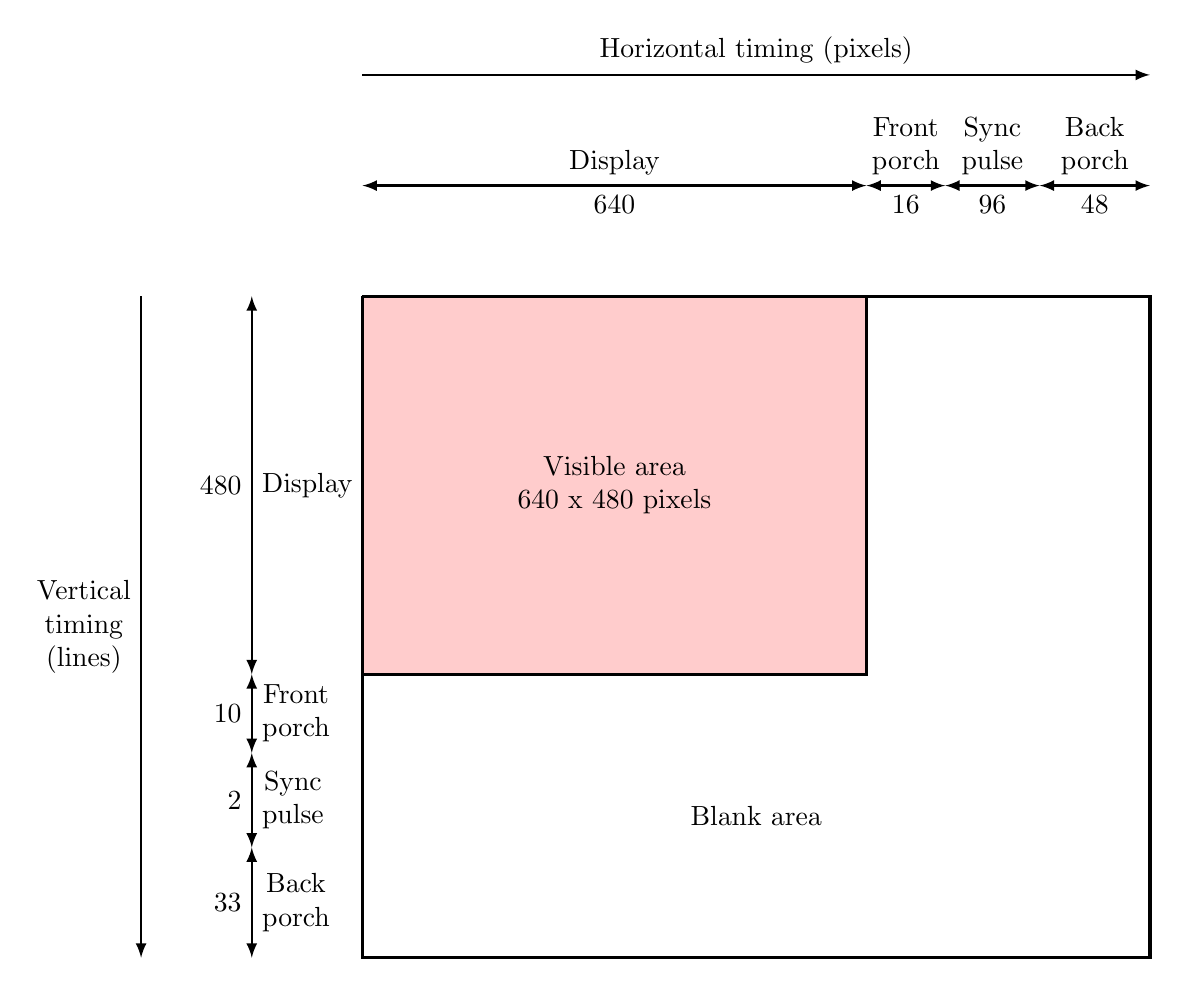
\begin{tikzpicture}

	\coordinate (origin) at (0,0);
	\coordinate (display) at (6.4,-4.8);
	\coordinate (front_porch) at (7.4,-5.8);
	\coordinate (sync_pulse) at (8.6,-7);
	\coordinate (back_porch) at (10,-8.4);

	\def\arrowSpacing{-40}

	% Visible area
	\draw[draw=black, very thick, fill=red!20]	(origin) -- 
														(origin |- display) -- 
														(display) -- 
														(origin -| display) -- 
														(origin);
	\draw[draw=none] (origin) -- node[midway,align=center]
		{Visible area\\ 640 x 480 pixels}(display);

	\draw[draw=none] (origin |- display) -- node[midway]{Blank area}(back_porch);
	% Blanking time
	\draw[draw=black,very thick]	(origin) -- 
																(origin |- back_porch) --
																(back_porch) --
																(origin -| back_porch) --
																(origin);

	% Horizontal timing
	\draw[draw,thick, latex-latex] 
		let 
			\p1=(origin),
			\p2=(display)
		in
		(\x1,{\y1-\arrowSpacing}) -- node[above,midway]{Display}
		node[below]{640}(\x2,{\y1-\arrowSpacing});
	
	\draw[draw,thick, latex-latex] 
		let 
			\p1=(origin),
			\p2=(display),
			\p3=(front_porch)
		in
		(\x2,{\y1-\arrowSpacing}) -- node[above,midway,align=center]{Front\\ porch}
		node[below]{16}(\x3,{\y1-\arrowSpacing});

	\draw[draw, thick, latex-latex] 
		let 
			\p1=(origin),
			\p2=(front_porch),
			\p3=(sync_pulse),
		in
		(\x2,{\y1-\arrowSpacing}) -- node[above,midway,align=center]{Sync\\ pulse}
		node[below]{96}(\x3,{\y1-\arrowSpacing});

		\draw[draw, thick, latex-latex] 
		let 
			\p1=(origin),
			\p2=(sync_pulse),
			\p3=(back_porch)
		in
		(\x2,{\y1-\arrowSpacing}) -- node[above,midway,align=center]{Back\\ porch}
		node[below]{48}(\x3,{\y1-\arrowSpacing});

	% Vertical timing
	\draw[draw,thick, latex-latex] 
		let 
			\p1=(origin),
			\p2=(display)
		in
		({\x1+\arrowSpacing},\y1) -- node[right,midway,align=center]{Display}
		node[left,midway]{480}({\x1+\arrowSpacing},\y2);
	
	\draw[draw,thick, latex-latex] 
		let 
			\p1=(origin),
			\p2=(display),
			\p3=(front_porch)
		in
		({\x1+\arrowSpacing},\y2) -- node[right,midway,align=center]{Front\\ porch}
		node[left,midway]{10}({\x1+\arrowSpacing},\y3);

	\draw[draw,thick, latex-latex] 
		let 
			\p1=(origin),
			\p2=(front_porch),
			\p3=(sync_pulse)
		in
		({\x1+\arrowSpacing},\y2) -- node[right,midway,align=center]{Sync\\ pulse}
		node[left,midway]{2}({\x1+\arrowSpacing},\y3);

	\draw[draw,thick, latex-latex] 
		let 
			\p1=(origin),
			\p2=(sync_pulse),
			\p3=(back_porch)
		in
		({\x1+\arrowSpacing},\y2) -- node[right,midway,align=center]{Back\\ porch}
		node[left,midway]{33}({\x1+\arrowSpacing},\y3);

	% Axis labels
	\draw[draw,thick, -latex] 
		let 
			\p1=(origin),
			\p3=(back_porch)
		in
		({\x1+2*\arrowSpacing},\y1) -- node[left,midway,align=center]{Vertical\\ timing\\ (lines)}
		({\x1+2*\arrowSpacing},\y3);

	\draw[draw, thick, -latex] 
		let 
			\p1=(origin),
			\p3=(back_porch)
		in
		(\x1,{\y1-2*\arrowSpacing}) -- node[above,midway,align=center]{Horizontal timing (pixels)}
		(\x3,{\y1-2*\arrowSpacing});	


\end{tikzpicture}
\end{document}
